\chapter{Radon Emanation in LZ}
\label{chap:chap4}

The discovery of radon dates back to 1900, when Friedrich Ernst Dorn reported results showing the emanation of a radioactive gas from radium compounds \cite{PARTINGTON1957}. Since then we now know that all isotopes of radon are radioactive, and only four are found in nature. With advancements in reducing cosmogenic and detector backgrounds in low-background dark matter experiments, emanation of radon is now the largest background contributor for the WIMP search RIO \cite{akerib2018projected}. The focus of this chapter is to highlight the relevance of radon for the LZ experiment; detailing the radon screening campaign of LZ, predominantly focusing on the work done at UCL and presenting the total expected radon emanation of the LZ detector.


%%------------------------------$$
\section{Overview}
%%------------------------------$$

Radon is a chemical element with an atomic number 86 found in the 6\textsuperscript{th} period of the noble gases. It occurs naturally in trace amounts in the radioactive decay chains through which uranium and thorium decay into lead and various other short-live radioactive elements, as shown in figure (\ref{fig:u_238_and_th_232}). It is found as a monatomic gas due to its full outer valence shell with solely radioactive isotopes. A consequence of its inert nature is that radon often exhibits a long diffusion length through solids. Its inert nature makes it extremely difficult for any filtration via chemical means, hence most removal attempts are achieved through physical methods. 

Radon is a colourless and odourless gas under standard temperature and pressure (STP). Its melting and boiling points are comparatively high for a noble gas, at -71\si{\degree} and -61.7\si{\degree}, respectively, and is densest of the noble gases with a density of 9.7 kg/\cubicmeter{}, and one of the most dense of all known gases. Activity of radon can vary substantially due to the composition of the environmental conditions. Typical atmospheric activities are $\sim10$ Bq/\cubicmeter{} and around 30--50 Bq/\cubicmeter{} for indoor environments. In underground laboratories, such as SURF, the activities can vary between 200--1000 Bq/\cubicmeter{} \cite{Heise_2015}, with significant fluctuations due to the variance in ventilation rate of the underground facility. Salt mines report amongst the lowest activities of all underground laboratories, such as the Boulby mine with $\sim3$ Bq/\cubicmeter{} \cite{scovell_boulby}. 

The significance of the radon background in LZ motivates a need for material screening and selection. \gray spectroscopy can help elude to the activities of \UandTe{} and \UandTl{}, but without material specific radon diffusion coefficients, it's difficult to understand the radon emanation rate of materials, purely from \gamma-spectroscopic results. LZ utilises on four facilities for radon emanation screening, built to collect and directly measure the emanated radon from screened samples, leading to a more accurate result in constructing the radon-induced background rate. The following sections will focus primarily on the operation of the UCL facility, highlighting important results measured for the LZ experiment. Thereafter, summaries of the other facilities will be detailed and the total radon budget of LZ will be taken into account. 

%%------------------------------$$
\section{Radon Backgrounds in LZ}
\label{sec:radon_and_lz}
%%------------------------------$$

\subsection{Origin of Radon Emanation}
\label{secsec:radon_origins}

All isotopes of radon are radioactive and only five are naturally found in minute quantities in nature. Those of interest for the LZ background model and often other low background experiments in search for WIMP dark matter or \neutrinolessDoubleBeta{} experiments are \RnTTT{} ($\tau_{1/2}=3.8232 \; d$) from the \UTTE{} decay chain and \RnTTZ{} ($\tau_{1/2}=55.8 \; s$) from the \ThTTT{} decay chain; hereafter called radon and thoron, respectively. Due to the long lifetime of their progenitor isotopes, radon and thoron are produced at a near-constant rate within detector material. They can then diffuse out, mixing with the GXe or LXe, and inevitably decaying within the active volume of the detector. The emanation rate of a material can be broken down into two parts: emanation due to recoiling radon atoms (i.e. \RnTTT{} or \RnTTZ{}) from their subsequent radium parent isotopes (i.e. \RaTTF{} or \RaTTS{}), $E_{recoil}$ and emanation due to diffusion, $E_{diffusion}$. The total emanation rate is then given the sum total of the two components,
%
\begin{equation}
    E_{tot} = E_{recoil} + E_{diffusion}.
    \label{eq:radon_emanation}
\end{equation}
%
Emanation due to diffusion can vary drastically depending on chemical and lattice structures of a material, density, surface roughness, and temperature; whereas the emanation from recoiling radon atoms depend heavily on the density of the material and the kinetic energy carried by the radon atom from the subsequent radium decay. \RnTTT{} (\RnTTZ{}) recoils with a kinetic energy of 86.26 (103.4) keV, with recoil ranges varying between 20--30 nm for materials such as Zircon or Quartz, and 60--65 \micro{}m for air and water \cite{radon_emanation_modeling}. The diffusion length, $L(m)$, is given as, 
%
\begin{equation}
    L(m) = \sqrt{D/\lambda},
    \label{eq:radon_emanation_diffusion}
\end{equation}
%
where $D$ is the diffusion coefficient and $\lambda{}$ the decay constant. A diffusion coefficient of $10^{-24} \; \MathText{m}^2 \; \MathText{s}^{-1}$ corresponds to  0.7($9 \times{} 10^{-3}$) nm for \RnTTT{} (\RnTTZ{}). Due to the much shorter half-life of \RnTTZ{}, the emanation of \RnTTZ{} in almost all material used in LZ is assumed to be dominated by the recoil emanation, whereas for \RnTTT{} both factors are assumed to play a role in the total emanation rate, with the ratio $E_{diffusion}/E_{recoil}$ expected to be suppressed in colder temperatures. 


\subsection{Radon Emanation Background in LZ}
\label{secsec:radon_in_lz}

In LZ, the material and surfaces of interest for radon emanation are those that are in direct contact with either GXe or LXe. Upon emanation, due to its relatively long half-life, \RnTTT{} is expected to mix homogeneously within the active volume. Although the same assumption is made for \RnTTZ{}, due to its much shorter half-life and diffusion length, a significant suppression is expected relative to \RnTTT{}, hence the assumed activity for \RnTTZ{} is 5\% that of the expected activity of \RnTTT{} as measured and estimated by radon screening. This assumption is made as a conservative measure as it's extremely difficult to screen for \RnTTZ{} emanation due to its short half-life.

The background from radon emanation for the WIMP search RIO is dominated by the ground-state to ground-state or \textit{naked} \beta-emission from the \PbTOF{} progeny of the \RnTTT{} sub-chain, as it decays to \BiTOF. This resulting in a uniform ER background with a \beta-spectrum of up to 1019 keV. Similarly, the background from \RnTTZ{} is from the \textit{naked} \beta-emission from \PbTOT{}, as it decays into \BiTOT{} with a \beta-spectrum of up to 569.9 keV. The remaining decays from the sub-radon chain are either too high in energy---in the case of \alpha-decays---or decay with a subsequent particle, i.e. a \gray{} or an \alpha particle, and hence can be vetoed via coincidence tagging, as such is the case for the \beta-decay of \BiTOF{}, which is subsequently followed by the \alpha-decay of \PbTOF{} with a half-life of $\tau{} = 162.3 \; \MathText{\micro{}s}$ \cite{radiogenic_muon_lux,Araujo:2011as}. The details of the decay of each isotope in the radon sub-chain are summarised in table (\ref{tab:radon_decay_chains}).

Radon emanation requirements for the LZ experiment are predetermined to ensure that the background due to radon does not significantly dominate over the irreducible \textit{pp} solar neutrino background, in order to maximise the potentiality of the WIMP search in the low mass region. A total of 20 mBq of \RnTTT{} activity is set as the threshold, of which 13.4 mBq is within the 7 tonnes of the active volume and 11.2 mBq in the 5.6 tonne fiducial volume. The radon emanation background from the latest projections as a result of the screening campaign accounts for $\sim66\%$ of the projected ER background in the WIMP search region of interest in LZ~\cite{akerib2018projected}, predominantly from a projected \RnTTT{}(\RnTTZ{}) specific activity of 1.83(0.09) {\micro\becquerel\per\kilogram} that corresponds to approximately \SI{18.3(0.9)} mBq in the 10 tonnes of xenon. The methodology used in estimating the projected activity of \RnTTT{} and \RnTTZ{} will be highlighted in later sections. 

\begin{table}[h]
\centering
\caption{Details of isotopes in the \RnTTT{} and \RnTTZ{} decay chains, starting from \RaTTS{} (upper) and \RaTTF{} (lower), down to \PoTOF{} and \PoTOT{}, respectively. The table also details the progenitor isotopes of the radon and thoron chains; \UTTE{} and \ThTTT{}.}
\label{tab:radon_decay_chains}
\vspace{1mm}
\renewcommand{\arraystretch}{1.2}
    \begin{tabular}{llllll}
    
    \textbf{Isotope} & %1
    \textbf{Decay} & %2
    \textbf{Q-value [MeV]} & %3
    \textbf{$\tau_{1/2}$} & %4
    & %4
    \textbf{Daughter} & %5
    
    \hline
    \hline
    
    \UTTE{}	    & \alpha{}      & 4.270     & 4.47($10^{9}$)  & y     & - \\ 
    \vdots      & \vdots        & \vdots    & \vdots          &       & \vdots \\ 
    \RaTTS{}	& \alpha{}      & 4.871     & 1600            & y     & \RnTTT{} \\ 
    \RnTTT{}	& \alpha{}      & 5.590     & 3.8232          & d     & \PoTOE{} \\ 
    \PoTOE{}	& \alpha{}      & 6.115     & 3.071           & m     & \PbTOF{} \\
    \PbTOF{}	& \beta{}       & 1.019     & 26.9            & m     & \BiTOF{} \\
    \BiTOF{}	& \beta{}       & 5.621     & 19.8            & m     & \PoTOF{} \\
    \PoTOF{}	& \alpha{}      & 7.833     & 162.3           & \micro{}s  & \PbTOZ{} \\
    
    \hline
    \hline
    
    \ThTTT{}	& \alpha{}      & 4.081     & 14.02($10^{9}$)   & y     & - \\ 
    \vdots      & \vdots        & \vdots    & \vdots            &       & \vdots \\ 
    \RaTTF{}	& \alpha{}      & 5.789     & 3.631             & d     & \RnTTZ{} \\ 
    \RnTTZ{}	& \alpha{}      & 6.405     & 55.8              & s     & \PoTOS{} \\ 
    \PoTOS{}	& \alpha{}      & 6.906     & 0.148             & s     & \PbTOT{} \\
    \PbTOT{}	& \beta{}       & 0.570     & 10.64             & h     & \BiTOT{} \\
    \BiTOT{}	& \beta{}       & 6.207     & 60.54             & m     & \PoTOT{} \\
    \PoTOT{}	& \alpha{}      & 8.954     & 300               & ns    & \PbTZE{} \\
    
    \bottomrule
    \end{tabular}
\end{table}




%%------------------------------$$
\section{UCL Radon Emanation System}
\label{sec:ucl_radon_system}
%%------------------------------$$

Material screening for radon emanation is often interpreted as the activity of radon released from the measured sample. Depending on the material at hand, the units are therefore either given in becquerels per surface area, mass or quantity of a given item. Most of the screening efforts are conducted on fractional quantities of the final material usage and the activities are scaled assuming to apply to the entirely of the material, provided they come from the same manufacturer and undergo the same cleanliness treatments as those screened.

Radon activity is reconstructed by measuring the radon sub-chain daughter isotopes, often \PoTOE{} and \PoTOF{}. Although commercial radon detectors are readily available---such as the Durridge Rad7 devices, their sensitivity is restricted to $~0.5$ Bq/\cubicmeter{}, which is orders of magnitude away from the sensitivity required for a reliable measurement of radon activities in the \micro{Bq}--mBq range, as required by LZ. The UCL radon emanation system utilises on a custom-made electrostatic detector, specially developed for use in many low background experiments. The following sections will briefly highlight the design and the operation of this system; outlining the detection technique, detector specifications and calibration measurements. More details on the construction of this system can be found in \cite{mott_2013, xin_2017}.


\subsection{Radon Detection \& Techniques}
\label{secsec:rn_detection_techniques}

The techniques involved in screening for radon generally reconstruct the radon emanation rate by measuring the radon sub-chain daughter isotopes. An indirect way of achieving this uses gamma spectroscopy to measure the \BiTOF{} and \PbTOF{} decay rates, from which the radon decay rate can be inferred. Although some useful constraints can be derived, it is extremely difficult to distinguish between radon daughters decaying in the bulk of the material and those that decay outside of the material, so emanation rates cannot be deduced without a material-specific diffusion model.

A more direct and accurate approach, one that has been utilised in the UCL system, is to directly measure the activity of radon that has emanated out of detector material. The sample material is initially enclosed in an air-tight chamber that is filled with a low-radon carrier gas, typically helium or nitrogen. This carrier gas prevents recoiling radon atoms from embedding themselves in the walls of the chamber.  After an emanation period that allows the radon concentration in the chamber to approach equilibrium, the emanated radon atoms are transferred into a detector that can either measure the rates of \PoTOE{} and \PoTOF{}. The emanation rate is reconstructed by correcting for the detection and transfer efficiencies, measured during dedicated runs with radon sources of known activity. 

The radon emanation rate is often determined by detecting the \alpha-particles of the radon progenies \PoTOE and \PoTOF{} in electrostatic detectors. These systems use electrostatic silicon PIN-diodes to attract and capture the predominantly positively charged ions (\SI{87.3\pm1.6}{\percent} \cite{PAGELKOPF20031057}) of radon daughter nuclei by using an electric field that is generated from the negative voltage applied on the PIN-diode \cite{CHOI2001177}. In using the progenies to reconstruct the emanation rate, it's important to understand the relationship between the activities of these isotopes to that of their parent isotope \RnTTT{}. In a radioactive decay chain, the number of atoms of a given isotope is dictated by the homeostasis between the number of atoms decaying from the parent isotope and those that are decaying into new daughter isotopes. When considering the decay chain, it is useful to introduce the following notation to identify the number of atoms and decay constant for each isotope:
%
\begin{align*}
    &^{222}\MathText{Rn} \;\; \rightarrow \;\; ^{218}\MathText{Po} \;\; \rightarrow \;\; ^{214}\MathText{Pb} \;\; \rightarrow \;\; ^{214}\MathText{Bi} \;\; \rightarrow \;\; ^{214}\MathText{Po} \\
    &N_{0}, \lambda{}_{0} \,\,\,\,\,\,\,\,\,\,\,\,\,\,
    N_{1}, \lambda{}_{1} \,\,\,\,\,\,\,\,\,\,\,\,\,\,
    N_{2}, \lambda{}_{2} \,\,\,\,\,\,\,\,\,\,\,\,\,\,
    N_{3}, \lambda{}_{3} \,\,\,\,\,\,\,\,\,\,\,\,\,\,
    N_{4}, \lambda{}_{4} 
    \label{eq:radon_decay_chain}
\end{align*}
%

The number of atoms of a given isotope in the chain can then be represented as 
%
\begin{equation}
    \frac{dN_{i}}{dt} = \lambda_{i-1}N_{i-1} - \lambda_{i}N_{i}
    \label{eq:isotopic_chance_in_chain}
\end{equation}
%
The activity of isotopes down the entire decay chain and its evolution with time can then be calculated by iteratively solving the above differential equation, provided $i=0$ represents \RnTTT{} and appropriate starting conditions are assumed; i.e. at $t=0$, $N_{0}= x \; \MathText{Bq}, \; N_{1-4} = 0$. The full deviation of activities down to \PoTOF{} can be found here \cite{mott_2013} and the evolution of activities of the chain starting from \RnTTT{} with an assumed activity of 1 mBq is shown in figure(\ref{fig:radon_chain_activity_evolution}).
%
\begin{figure}[t!]
    \centering
    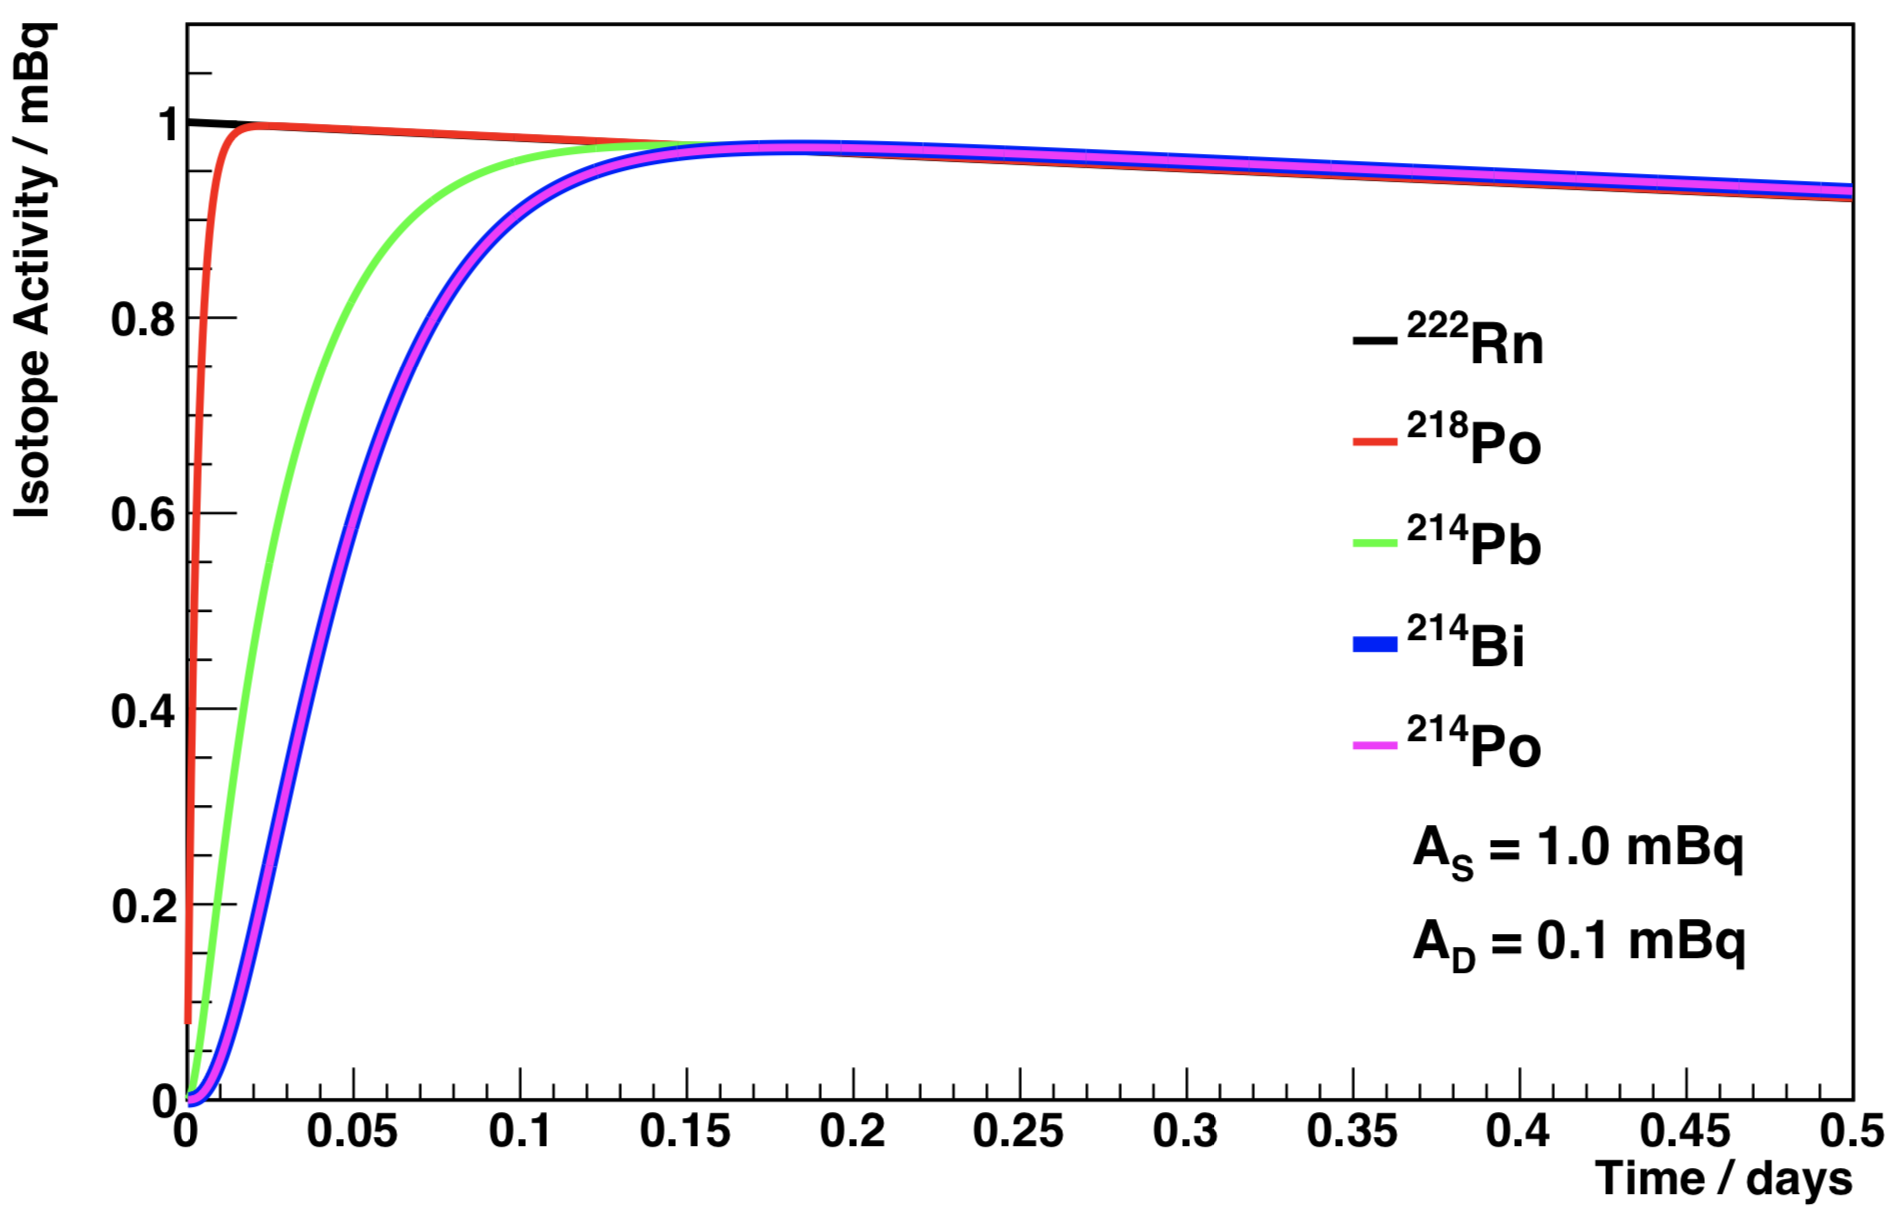
\includegraphics[scale=0.40]{Chapter_4/Figures/radon_chain_activities.png}
    \caption[The evolution of activities of the \RnTTT{} decay chain with respect to time under the starting condition of 1 mBq of \RnTTT{}.]
    {The evolution of activities of the \RnTTT{} decay chain with respect to time under the starting condition of 1 mBq of \RnTTT{}. $A_{D}$ represents the intrinsic background activity of the detector. Figure adapted from \cite{mott_2013}.}
    \label{fig:radon_chain_activity_evolution}
\end{figure}
%
Its important to note that the activity of \PoTOE{} quickly reaches an equilibrium with \RnTTT{}, whereas it takes $\sim4.5$ hours for \PoTOF{}. Hence, this slight delay needs to be taken into account if the emanation from a sample is transferred into the detector prior to equilibrium. Provided equilibrium is reached, the measured activity of both \PoTOE{} and \PoTOF{} will be equivalent to the activity of \RnTTT{}.


\subsection{Electrostatic Detector}
\label{secsec:electrostatic_detector}



\subsection{Detector Efficiency}
\label{secsec:rn_detection_techniques}



\subsection{Radon Concentration Line}
\label{secsec:concentration_line}






\section{UCL Radon Measurements for LZ}
\label{sec:uclradon}


\section{Other Radon Emanation Assays for LZ}
\label{sec:otherradon}


\section{Radon Emanation Background in LZ}
\label{sec:lzradon}

\section{Conclusion}